\section{Results}\label{sec:results}

\subsection{Employment in Selected Occupations}\label{sec:results:occupations}

Figure~\ref{fig:occupations_by_age} displays normalized employment per capita for four occupation groups with high theoretical AI exposure: software developers, ICT systems analysts, customer service agents, and ICT operations technicians.\footnote{ISCO-08 codes: software developers 2512--2514 and 2519; ICT systems analysts 2511; customer service agents 4222; ICT operations technicians 3511.} Each panel plots employment per capita indexed to October 2022 = 1, separately by age group, with a vertical line marking the public release of ChatGPT on November 30, 2022.

The gradient is largest in software development. The 22--25 series falls from 1.0 at the index date to about 0.70 by late 2025; the 35--40 series rises to 1.15 over the same window. The 26--30 series also falls, less steeply. ICT systems analysts look the same: 22--25 down to 0.75, 35--40 up to 1.10.

Customer service agents show the same age gradient, with more month-to-month variation. The 22--25 group fluctuates around 0.95 before declining toward the end of the period, while the 31--40 groups grow to approximately 1.10--1.15. ICT operations technicians exhibit a weaker version of the pattern: the youngest group declines modestly to around 0.90, and the age separation is less pronounced than in the other three panels.

All four occupations rank high on AI exposure indices and feature in similar case studies in \citet{brynjolfsson2025}; in all four the youngest workers lose ground while older workers do not. Section~\ref{sec:results:quintiles} incorporates all occupations systematically.

\begin{figure}[tp]
  \centering
  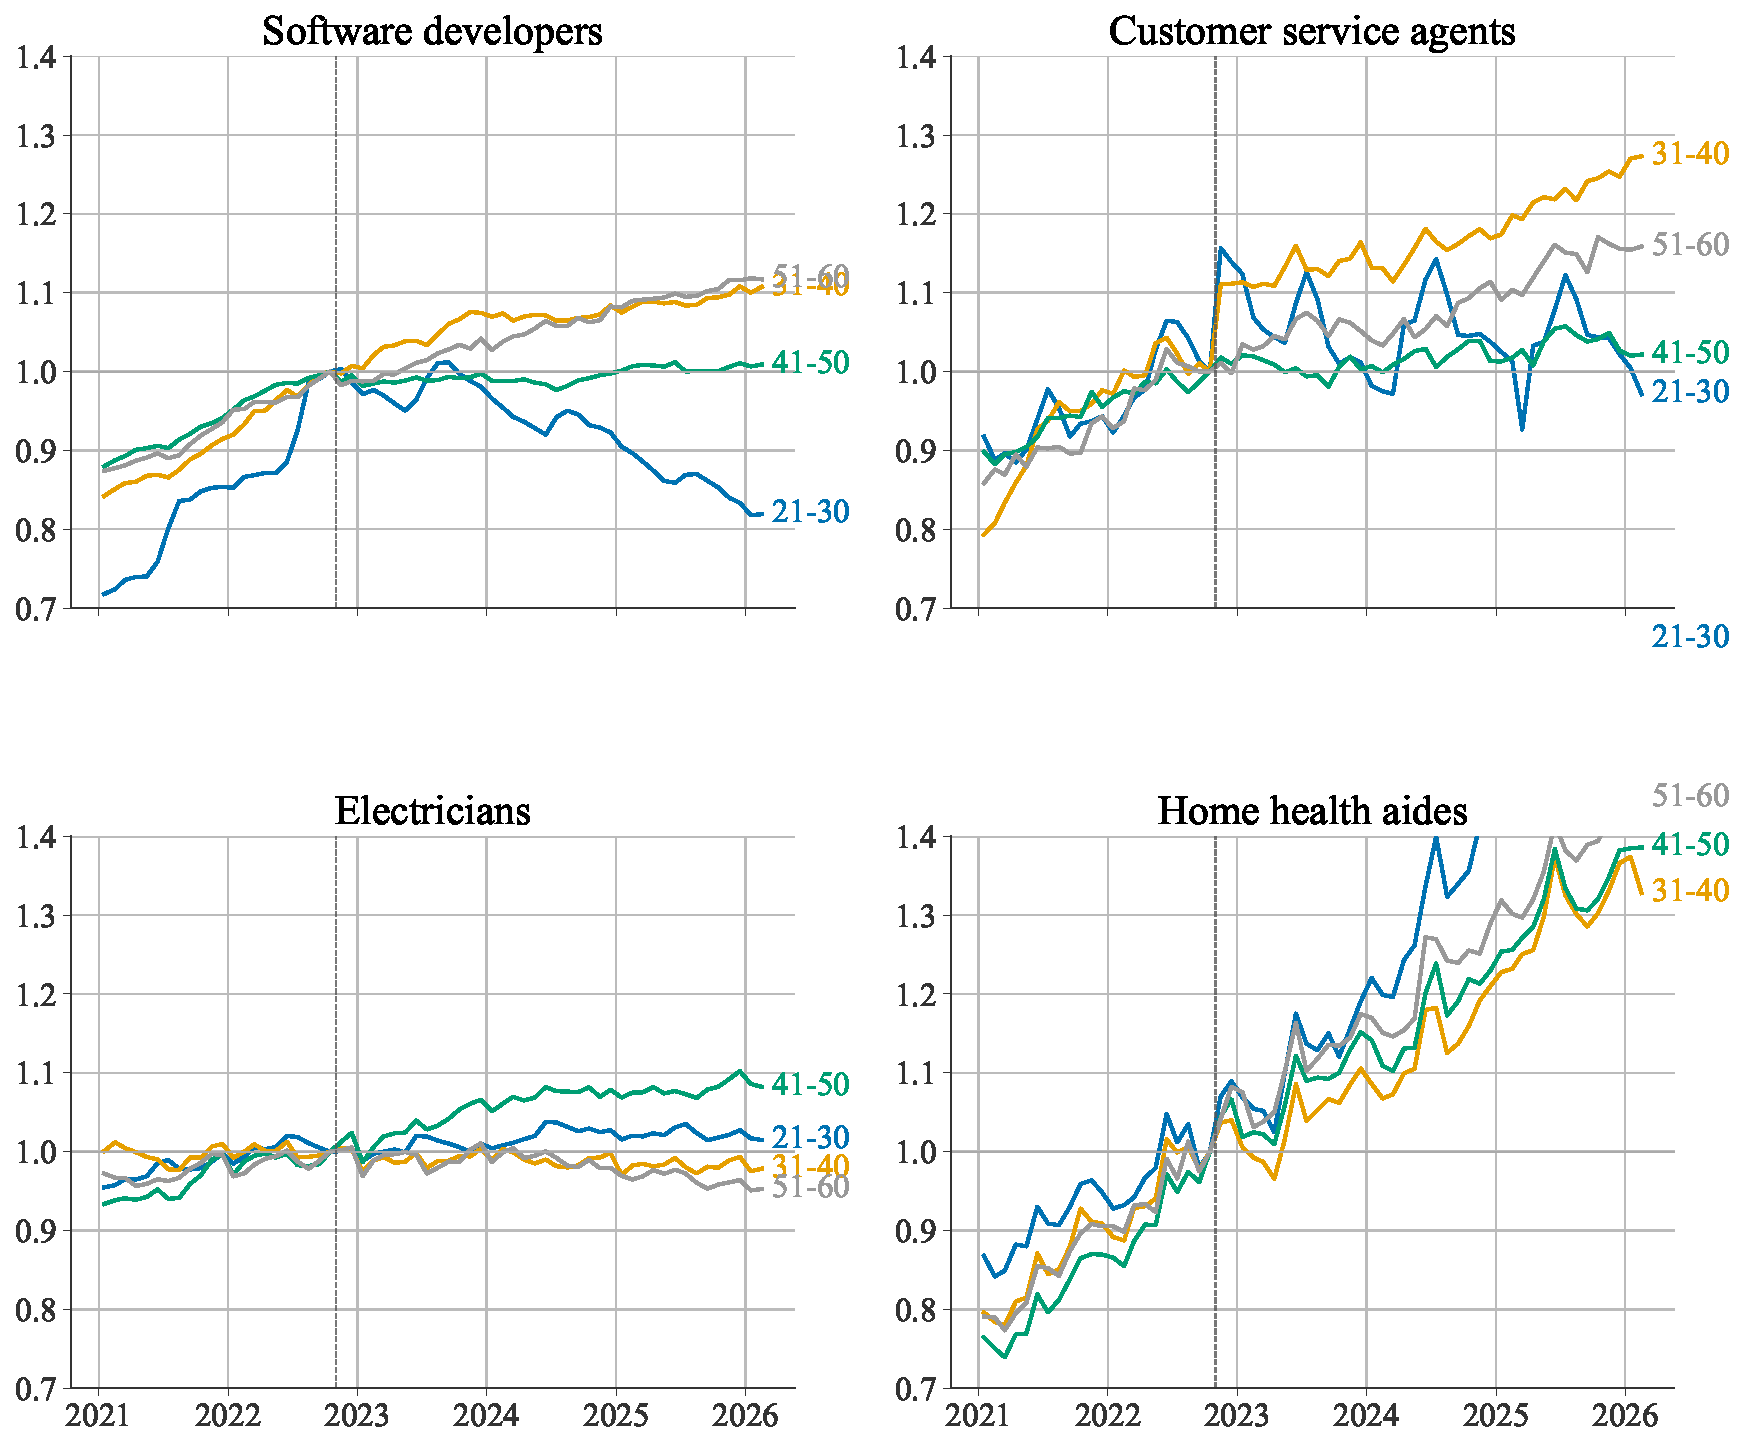
\includegraphics[width=\textwidth]{../analysis/output/figures/figure1_occupations_by_age.pdf}
  \caption{Employment per capita (October 2022 = 1) by age group for selected high-exposure occupations. Employment counts divided by population in each age group (SSB table 07459) with composition adjustment (reference: 2021-Q1). Panels show software developers (ISCO-08 2512--2514, 2519), ICT systems analysts (2511), customer service agents (4222), and ICT operations technicians (3511). The vertical dashed line marks November 30, 2022 (ChatGPT release).}
  \label{fig:occupations_by_age}
\end{figure}


\subsection{Employment by AI Exposure Quintile}\label{sec:results:quintiles}

The case studies above examine occupations chosen for their AI relevance. A more systematic approach ranks all occupations by their AI exposure score and examines whether high-exposure occupations exhibit different employment trends than low-exposure occupations. We assign each occupation to a quintile based on its Eloundou et al.\ GPT-4 exposure score, from Q1 (least exposed) to Q5 (most exposed), and plot normalized employment by quintile within each age group.

\subsubsection*{Eloundou et al.\ Exposure}

Figure~\ref{fig:age_by_quintile} plots quintile-by-age normalized employment per capita. The figure contains six panels, one per age group, with quintile lines running from light blue (Q1, least exposed) to dark blue (Q5, most exposed) and a red line for the overall age-group trend.

At ages 22--25 the quintiles separate after the ChatGPT release. Q5 falls from 1.0 to 0.85--0.90 by 2025; Q1 stays flat. Q4, Q3, and Q2 fall less steeply, in that order. The overall (red) line slopes down, with the decline concentrated in the upper quintiles.

As noted above, software developers aged 22--25 decline by roughly 30 percent, yet Q5 as a whole declines by only about 10 percent. The discrepancy reflects within-quintile heterogeneity. Software development occupations account for approximately 2,300 of the 29,500 workers aged 22--25 in Q5 (about eight percent). The largest Q5 occupations are office workers and service occupations: general office clerks (approximately 5,500 workers) decline by about 21 percent, but insurance agents, policy advisors, and receptionists are roughly stable. Several Q5 occupations grow: insurance representatives ($+39$ percent), sales workers ($+32$ percent), and accountants ($+25$ percent). The net result is a moderate aggregate decline that masks heterogeneity across occupations within the same exposure quintile.\footnote{ISCO-08 codes: software development 2512--2514 and 2519; general office clerks 4110; insurance agents 3322; policy advisors 2422; receptionists 4226; insurance representatives 3321; sales workers 5249; accountants 3313.}

\citet{gans2025} and \citet{imas2026} argue on theoretical grounds that average task exposure is a poor predictor of actual adjustment when tasks are complements rather than substitutes. Under this view, many high-exposure occupations should be augmented rather than displaced. If that were the main explanation for the within-Q5 heterogeneity, we would expect a sharper gradient when occupations are ranked by their automation share (Section~\ref{sec:results:auto_aug}) rather than by overall exposure. The Handa et al.\ automation quintiles (Appendix Figure~\ref{fig:age_by_quintile_handa_auto}) do show a gradient for 22--25 year-olds, but it is not substantially stronger than the overall exposure gradient. A direct test of the O-ring / job-dimensionality prediction is reported in Appendix Figure~\ref{fig:dimensionality}. The results are inconclusive. Either the Handa measure's limited task coverage and conversation-structure basis (Section~\ref{sec:literature}) prevent it from cleanly separating automation from augmentation, or many high-exposure occupations have not yet been touched by adoption regardless of their theoretical exposure. The quintile gradient averages over this heterogeneity.

The 26--30 panel has the same shape with smaller magnitudes: Q5 still ends below Q1 by 2025, but the spread narrows and the separation starts later. From age 31 upward the gradient disappears. Ages 31--34 and 35--40 grow from 0.9 toward 1.05 across all quintiles, with Q5 at least keeping pace with Q1, a pattern compatible with firms substituting toward early-thirties workers when entry-level hiring in exposed occupations slows. Ages 41--49 and 50+ track each other across quintiles with a mild upward drift.

Thus, there is a decline among the youngest workers in the most-exposed occupations. Adjustment that operates through hiring rather than separations fits this age profile. 


\begin{figure}[tp]
  \centering
  
\includegraphics[width=\textwidth]{../analysis/output/figures/figure2_age_by_quintile.pdf}
  \caption{Employment per capita (October 2022 = 1) by Eloundou et al.\ GPT-4 exposure quintile and age group. Employment counts divided by population in each age group with composition adjustment (reference: 2021-Q1). Q1 (lightest) = least exposed; Q5 (darkest) = most exposed. Red line = overall age-group trend. Vertical dashed line marks ChatGPT release.}
  \label{fig:age_by_quintile}
\end{figure}

\subsubsection*{Felten AIOE Exposure}

Figure~\ref{fig:age_by_quintile_felten} repeats the quintile analysis with the \citet{felten2021} AIOE index. The 22--25 panel matches the Eloundou figure, with Q5 below Q1 and the same monotone ordering, as the two measures correlate at $\rho = 0.889$ (Table~\ref{tab:correlations}). Older ages again show no gradient.

\begin{figure}[tp]
  \centering
  
\includegraphics[width=\textwidth]{../analysis/output/figures/figure9a_age_by_quintile_felten.pdf}
  \caption{Employment by Felten et al.\ AIOE quintile and age group.}
  \label{fig:age_by_quintile_felten}
\end{figure}

\subsubsection*{Handa et al.\ Overall Exposure}

Figure~\ref{fig:age_by_quintile_handa} uses quintiles based on the \citet{handa2025} overall exposure measure, which captures revealed patterns of Claude usage rather than theoretical capability. The pattern for 22--25 year-olds is present but weaker. Q5 separates from the other quintiles, but the spread is smaller than in the Eloundou et al.\ and Felten et al.\ figures. The quintile ordering is less cleanly monotonic, with intermediate quintiles sometimes crossing.

Older age groups again show no gradient. The Handa et al.\ measure reflects how workers actually use Claude, not how exposed their occupations are in principle, and Claude usage is concentrated in a narrow set of task types (Section~\ref{sec:data:ai}). The weaker employment signal under revealed-usage quintiles could reflect either early-stage adoption or a gap between theoretical capability and actual workplace use.

\begin{figure}[tp]
  \centering
  
\includegraphics[width=\textwidth]{../analysis/output/figures/figure5a_age_by_quintile_handa.pdf}
  \caption{Normalized employment (October 2022 = 1) by Handa et al.\ overall exposure quintile and age group. Q1 (lightest) = least exposed; Q5 (darkest) = most exposed. Red line = overall age-group trend.}
  \label{fig:age_by_quintile_handa}
\end{figure}

The companion automation and augmentation quintile plots based on the Handa et al.\ decomposition are reported in Appendix Figures~\ref{fig:age_by_quintile_handa_auto} and~\ref{fig:age_by_quintile_handa_aug}; the time-weighted \citet{anthropic2026} \texttt{job\_exposure} version is in Appendix Figure~\ref{fig:age_by_quintile_job_exposure}.


\subsection{Automation versus Augmentation}\label{sec:results:auto_aug}

We follow \citet{brynjolfsson2025} on the automation-vs-augmentation split. Ranking 22--25-year-olds by Handa automation share gives a modest negative gradient (Appendix Figure~\ref{fig:age_by_quintile_handa_auto}); ranking them by augmentation share gives no gradient at all (Appendix Figure~\ref{fig:age_by_quintile_handa_aug}). The split points toward displacement rather than augmentation, but the Handa classification only captures conversation mode, not what workers actually do on the job. An occupation scored as ``automation-exposed'' through conversation mode may in practice use AI for augmentation. 


\subsection{Sector Heterogeneity}\label{sec:results:sectors}

Figure~\ref{fig:sector_by_quintile} decomposes the employment quintile analysis by institutional sector. The three panels show the private sector, the municipal sector, and the state sector, with Eloundou et al.\ quintile lines plotted for each.

When all age groups are pooled, no quintile gradient is visible in any of the three sectors: workers aged 22--25 are a small share of total employment, so the age-specific gradient documented in Figure~\ref{fig:age_by_quintile} washes out in the pooled series. When broken down by sector (Appendix Figures~\ref{fig:sector_private_age}--\ref{fig:sector_state_age}), the age-exposure gradient reappears in the private sector but is absent in the municipal and state sectors.

The public-sector null could reflect slower adoption, hiring insulated from market conditions, stronger employment protection, or a different occupational mix; we cannot separate these from the aggregate data. The adoption channel does have some support: \citet{riksrevisjonen2024} report that more than half of Norwegian state agencies have no experience with AI tools, so theoretical exposure in the public sector does not translate into implementation. The public sector is dominated by health, education, and administration; private high-exposure occupations cluster in IT, finance, and business services. 

\begin{figure}[tp]
  \centering
  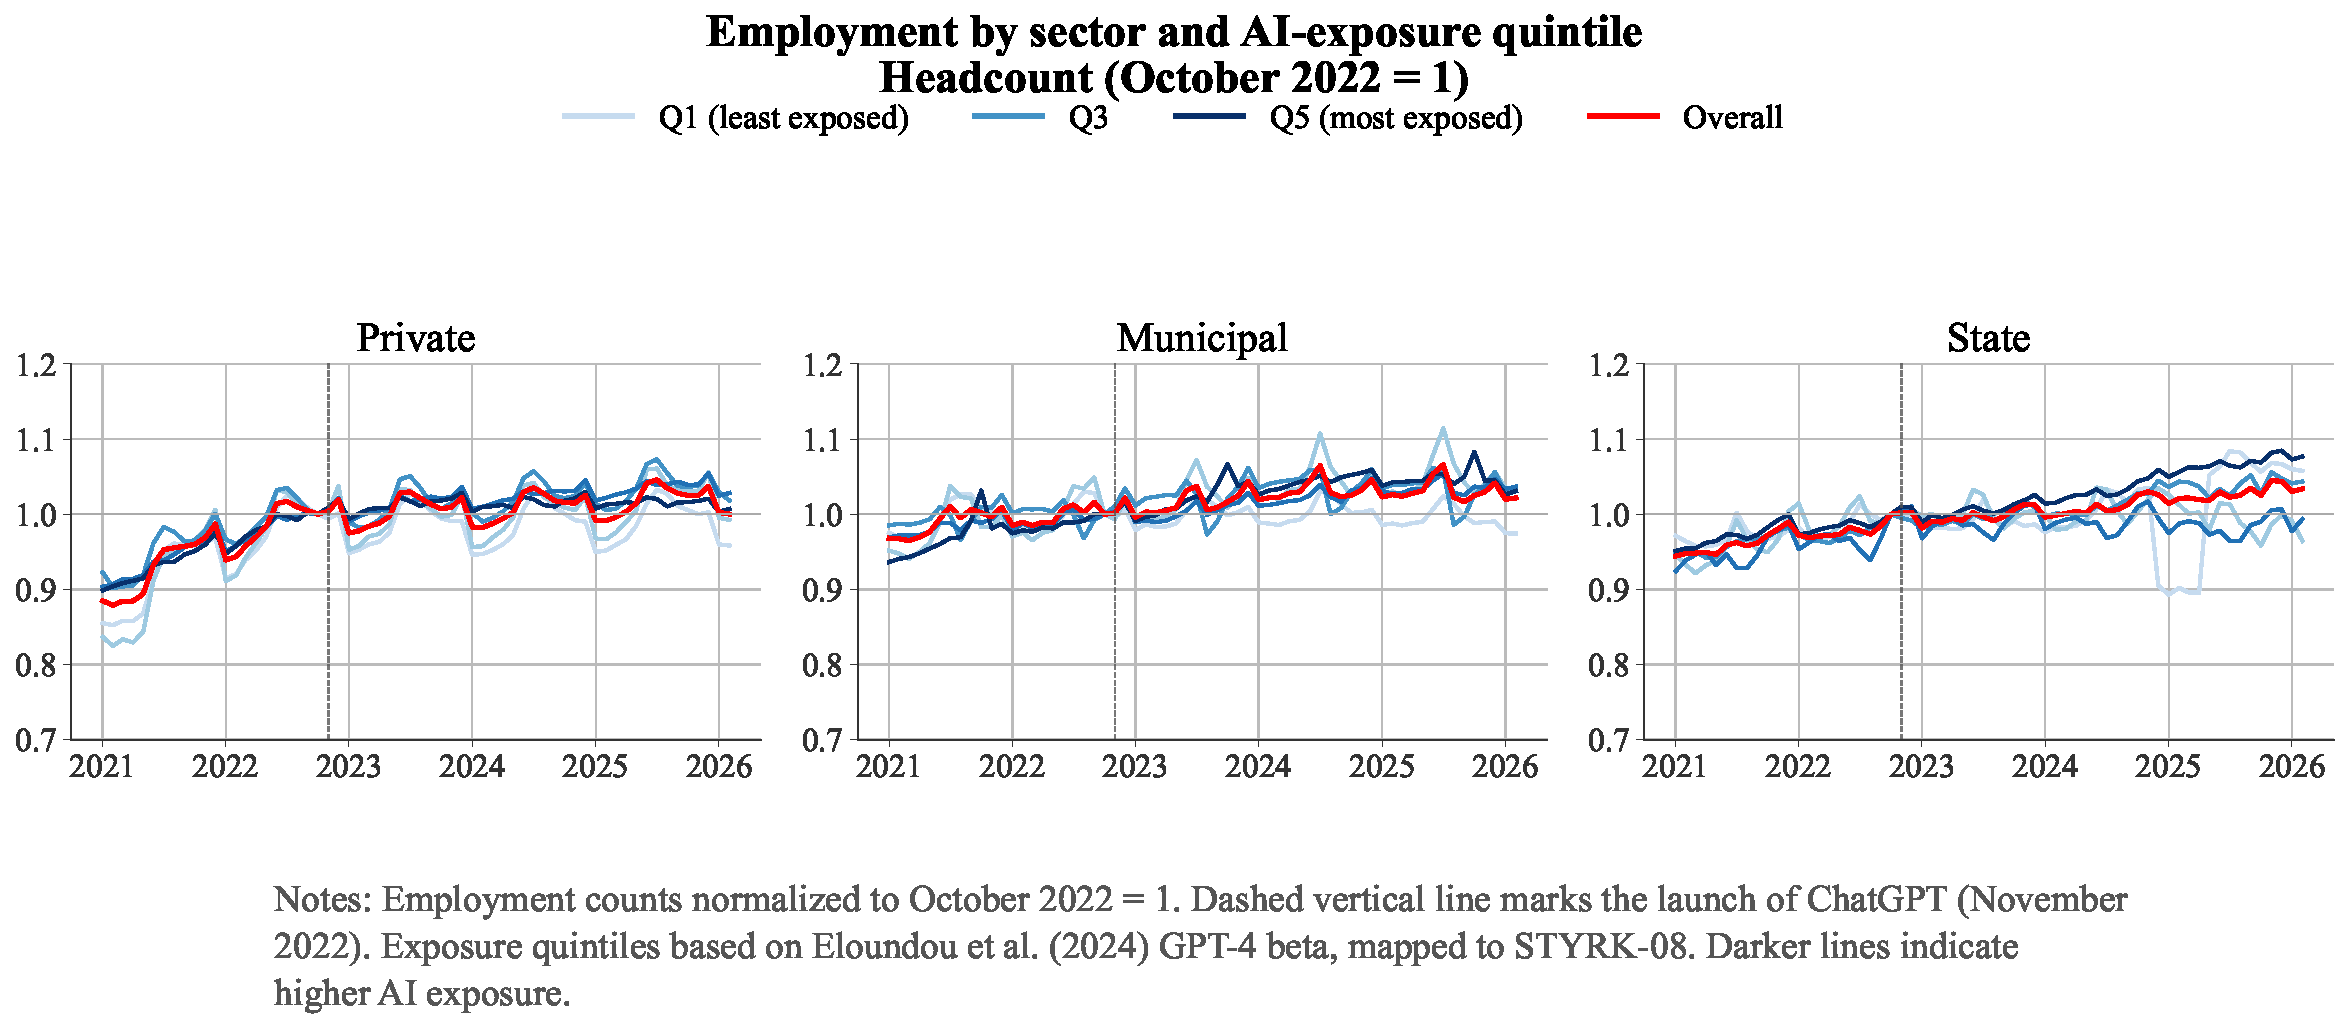
\includegraphics[width=\textwidth]{../analysis/output/figures/figure3_sector_by_quintile.pdf}
  \caption{Employment by Eloundou et al.\ exposure quintile, decomposed into private, municipal, and state sectors.}
  \label{fig:sector_by_quintile}
\end{figure}


\subsection{Wages and Other Outcomes}\label{sec:results:wages}

Figure~\ref{fig:kontantlonn_by_quintile} displays monthly cash earnings by Eloundou et al.\ exposure quintile and age group. Strong seasonal patterns dominate the wage plots: December earnings spike to 1.4--1.5 times the baseline due to Christmas bonuses, and June earnings are elevated due to statutory holiday pay. \citet{brynjolfsson2025} and \citet{humlum2026} find no wage divergence over a similar horizon in the US and Denmark. Norway's two-tier bargaining system \citep{bhuller2022} with sectoral wage floors and strong employment protection make the quantity margin the more likely site of adjustment.

Four additional outcomes are reported in the appendix: hourly wages (Figure~\ref{fig:timelonn_by_quintile}), contracted position percentage (Figure~\ref{fig:stillingspst_by_quintile}), overtime hours (Figure~\ref{fig:overtid_by_quintile}), and the share of new jobs (Figure~\ref{fig:nyjobb_by_quintile}). None shows a differential trend by exposure quintile, consistent with the extensive margin as the candidate site of adjustment.

\begin{figure}[tp]
  \centering
  
\includegraphics[width=\textwidth]{../analysis/output/figures/figure7a_kontantlonn_by_quintile.pdf}
  \caption{Normalized monthly cash earnings (October 2022 = 1) by Eloundou et al.\ exposure quintile and age group. Strong seasonal patterns (December bonuses, June holiday pay) are visible in all panels. No systematic divergence between high- and low-exposure quintiles emerges in any age group.}
  \label{fig:kontantlonn_by_quintile}
\end{figure}


\subsection{Poisson Regression Estimates and Within-Firm Reallocation}\label{sec:results:firmfe}

The quintile series so far normalize employment by the population in each age group, the right denominator for asking whether cohort-level employment shifts away from AI-exposed occupations. We turn now to the worker counts and ask if they reallocate across occupations? Following \citet{brynjolfsson2025}, we estimate Poisson event studies on the counts.

We report two specifications. The first uses the cell-level aggregates that underlie the rest of Section~\ref{sec:results}; it covers the universe of formal employment and includes any composition shifts \emph{between} firms. The second uses individual-level employer-reported records, restricted to private-sector firms with at least 20 workers in the age window over the full 2021m1--2025m7 panel, and adds firm fixed effects to remove between-firm composition. The two are not nested: they differ in sample (universe vs.\ panel-balanced private-sector firms above the size threshold), in identifying variation (within-occupation time variation vs.\ within-firm-by-quintile time variation), in implicit Poisson weighting (by occupation size vs.\ by firm-by-quintile cell size), and in clustering unit (occupation vs.\ firm). Differences between them therefore to some extent mix between-firm reallocation with sample selection and the choice of FE level. We discuss both below.

\paragraph{Cell-level.}
The cell-level microdata are tabulated at the (occupation $\times$ age bin $\times$ month) level. We estimate
\[
\log E[\text{count}_{j,a,t}] = \alpha_{j} + \beta_{t} + \gamma_{q,k},
\]
separately per age bin~$a$, where $j$ indexes occupations and $q(j)$ is the Eloundou GPT-4 $\beta$ quintile of occupation~$j$. The occupation FE absorbs the permanent employment level of each occupation; the month FE absorbs the aggregate time path of the age cohort. Standard errors are clustered at occupation. Reference: Q1 and $k=-1$ (October 2022).

Figure~\ref{fig:microdata_poisson_grid} reports the resulting $\gamma_{q,k}$ for $q\in\{2,3,4,5\}$ across the six age bins, in log points. The same picture emerges as in the linear rate figure (Figure~\ref{fig:age_by_quintile}). At 22--25, Q5 reaches $-15$ to $-20$ log points by 2025, Q3 and Q4 fall less steeply, and Q2 is flat to slightly negative; the ordering is monotone. The 26--30 panel has the same sign at smaller magnitude. From age 31 upward, the gradient flattens or reverses, with Q5 growing slightly above Q1 in the mid-career bins.

\begin{figure}[tp]
  \centering
  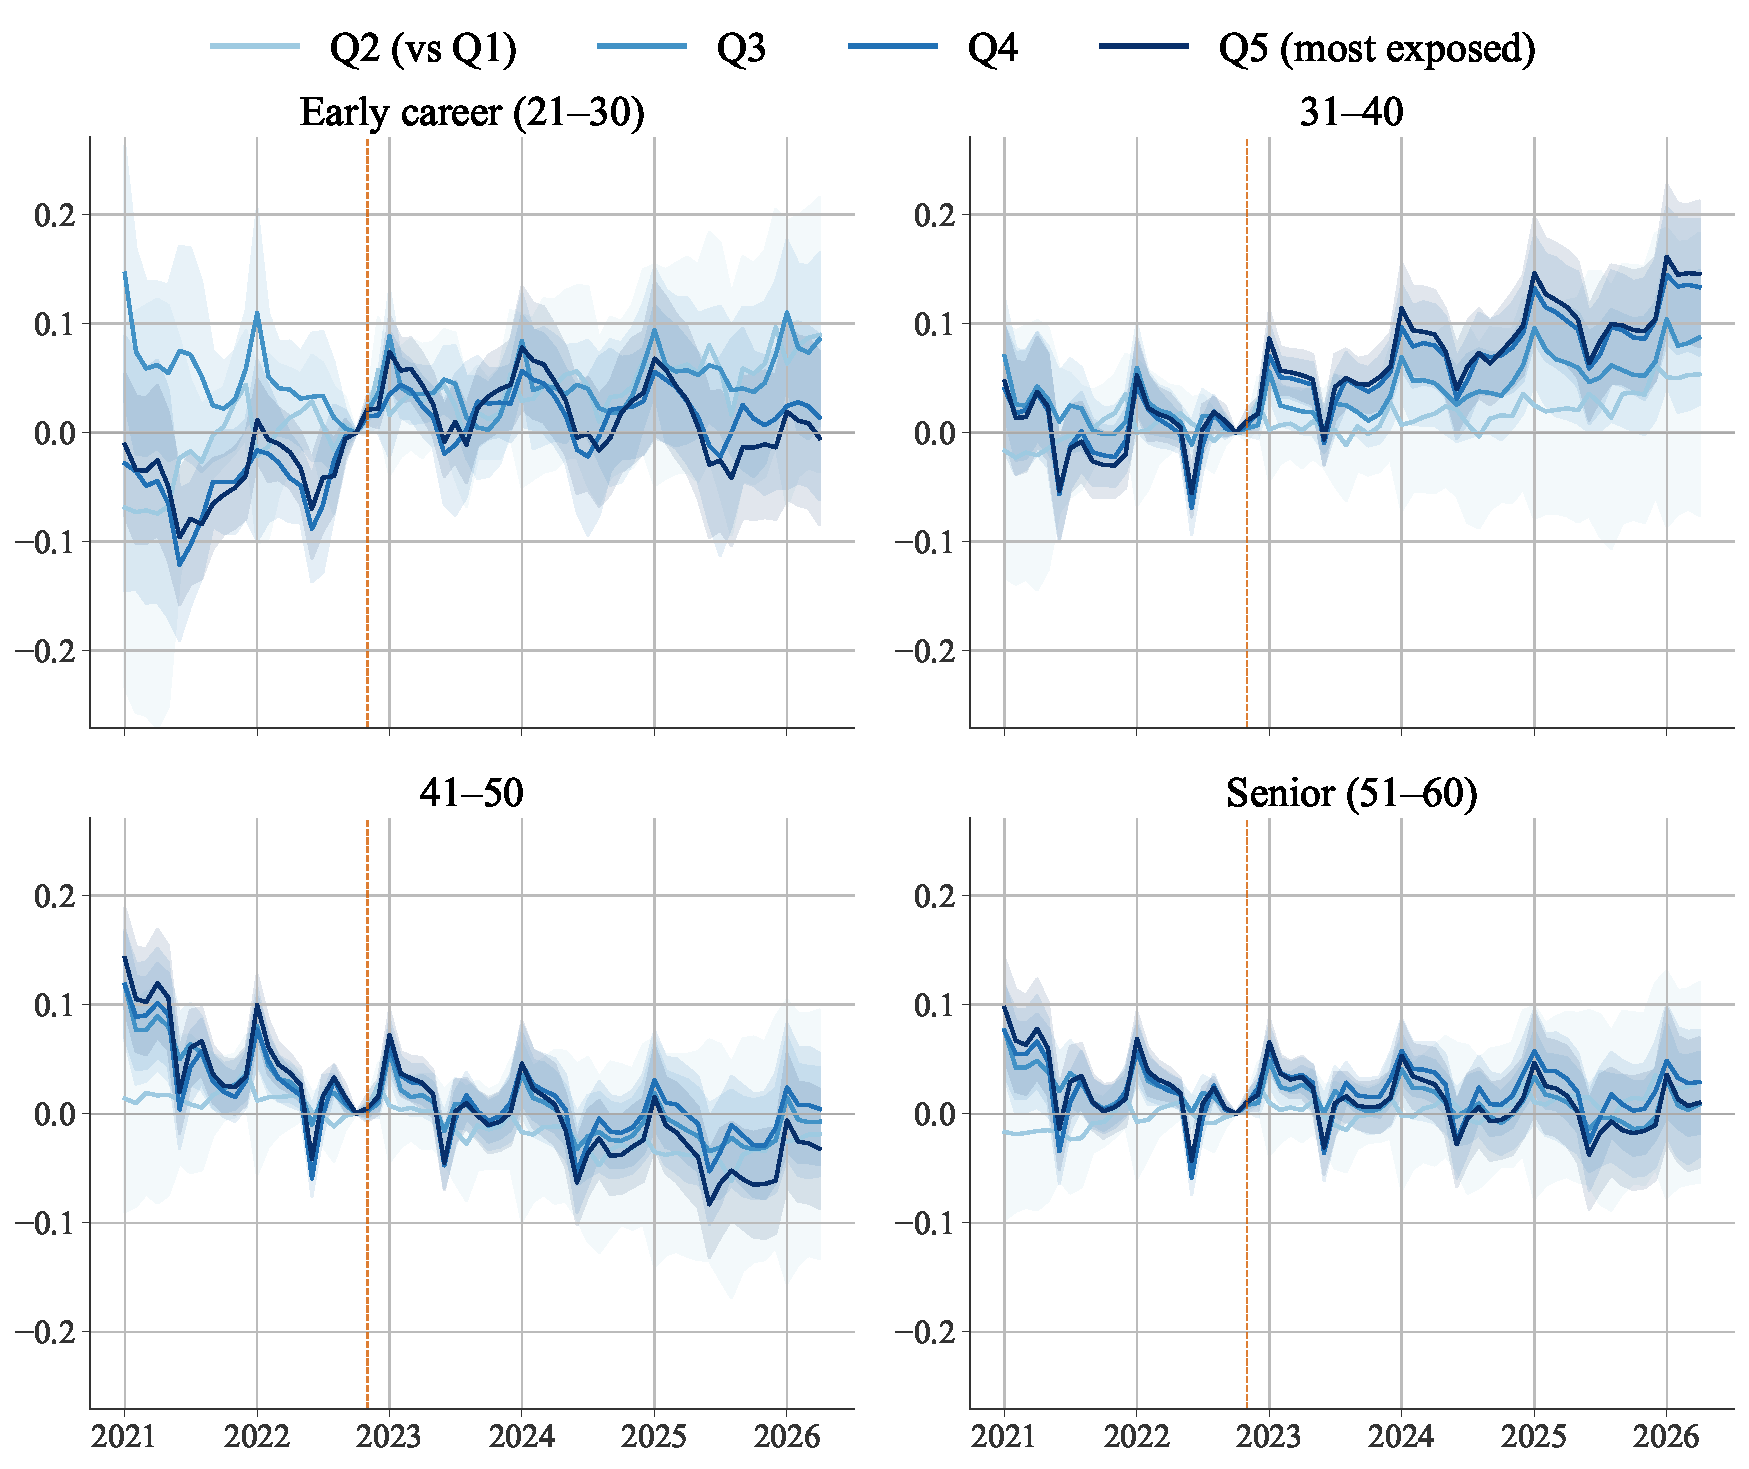
\includegraphics[width=\textwidth]{../analysis/output/figures/figure_microdata_poisson_es_grid.pdf}
  \caption{Poisson event-study coefficients $\gamma_{q,k}$ for $q\in\{2,\dots,5\}$ vs.\ $q=1$, by age bin. Cell-level microdata.no aggregates (occupation\,$\times$\,age\,$\times$\,month); FE: occupation and month. Sample: 22--55-year-olds, 2021m1--2025m7. Shaded band: 95\% CI clustered at occupation. Reference: October 2022. Dashed red line: November 2022 (ChatGPT release).}
  \label{fig:microdata_poisson_grid}
\end{figure}

\paragraph{Within-firm.}
The individual-level records are available to us only through July 2025, six months short of the cell-level series we use for the main analysis. For that reason we do not adopt the within-firm specification as our headline design. We run it here as a check on the aggregated results: if the cohort-level pattern documented above were driven by reorganization \emph{within} continuing firms, that should show up in a within-firm composition specification \`{a} la \citet{brynjolfsson2025}.

The panel covers private-sector firms from 2021m1 through 2025m7, restricted to ages 22--55 with positive cash earnings and a valid occupation code. We keep firms with at least 20 workers in the age window, fill synthetic zeros for (firm, age bin, occupation) cells ever observed, and rank occupations into quintiles on Eloundou et al.\ GPT-4 $\beta$. The estimating sample is 48.8 million worker-months across 18{,}400 firms. The unit of observation is the (firm, age bin, quintile, month) cell; the outcome is the count of workers in that cell. A firm is not assigned to a quintile, it typically employs workers across several occupations spanning multiple quintiles, and what firms differ in is the \emph{share} of employment in each quintile. We estimate with firm-by-quintile and firm-by-month fixed effects separately per age bin:
\[
\log E[\text{count}_{f,q,a,t}] = \alpha_{f,q} + \beta_{f,t} + \gamma_{q,k},
\]
with reference $k=-1$ and standard errors clustered at firm. The firm-by-quintile FE absorbs each firm's permanent employment level in each quintile (so heterogeneity in firms' occupational mix is netted out); the firm-by-month FE absorbs each firm's overall employment trajectory. The remaining variation identifies, within a firm and age bin, whether Q5 employment evolves differently from Q1 employment after October 2022.

Figure~\ref{fig:firmfe_poisson_grid} reports the same Q2--Q5 vs.\ Q1 grid for the firm-FE specification. The 22--25 panel is centered near zero with wide CIs and no break at November 2022; the cell-level grid in Figure~\ref{fig:microdata_poisson_grid} reaches $-15$ to $-20$ log points in the same panel. Ages 26--30 through 35--40 drift up to $+8$ to $+10$ log points by mid-2025, monotone in exposure. Ages 41--49 and 50--55 are flat to slightly negative.

\begin{figure}[tp]
  \centering
  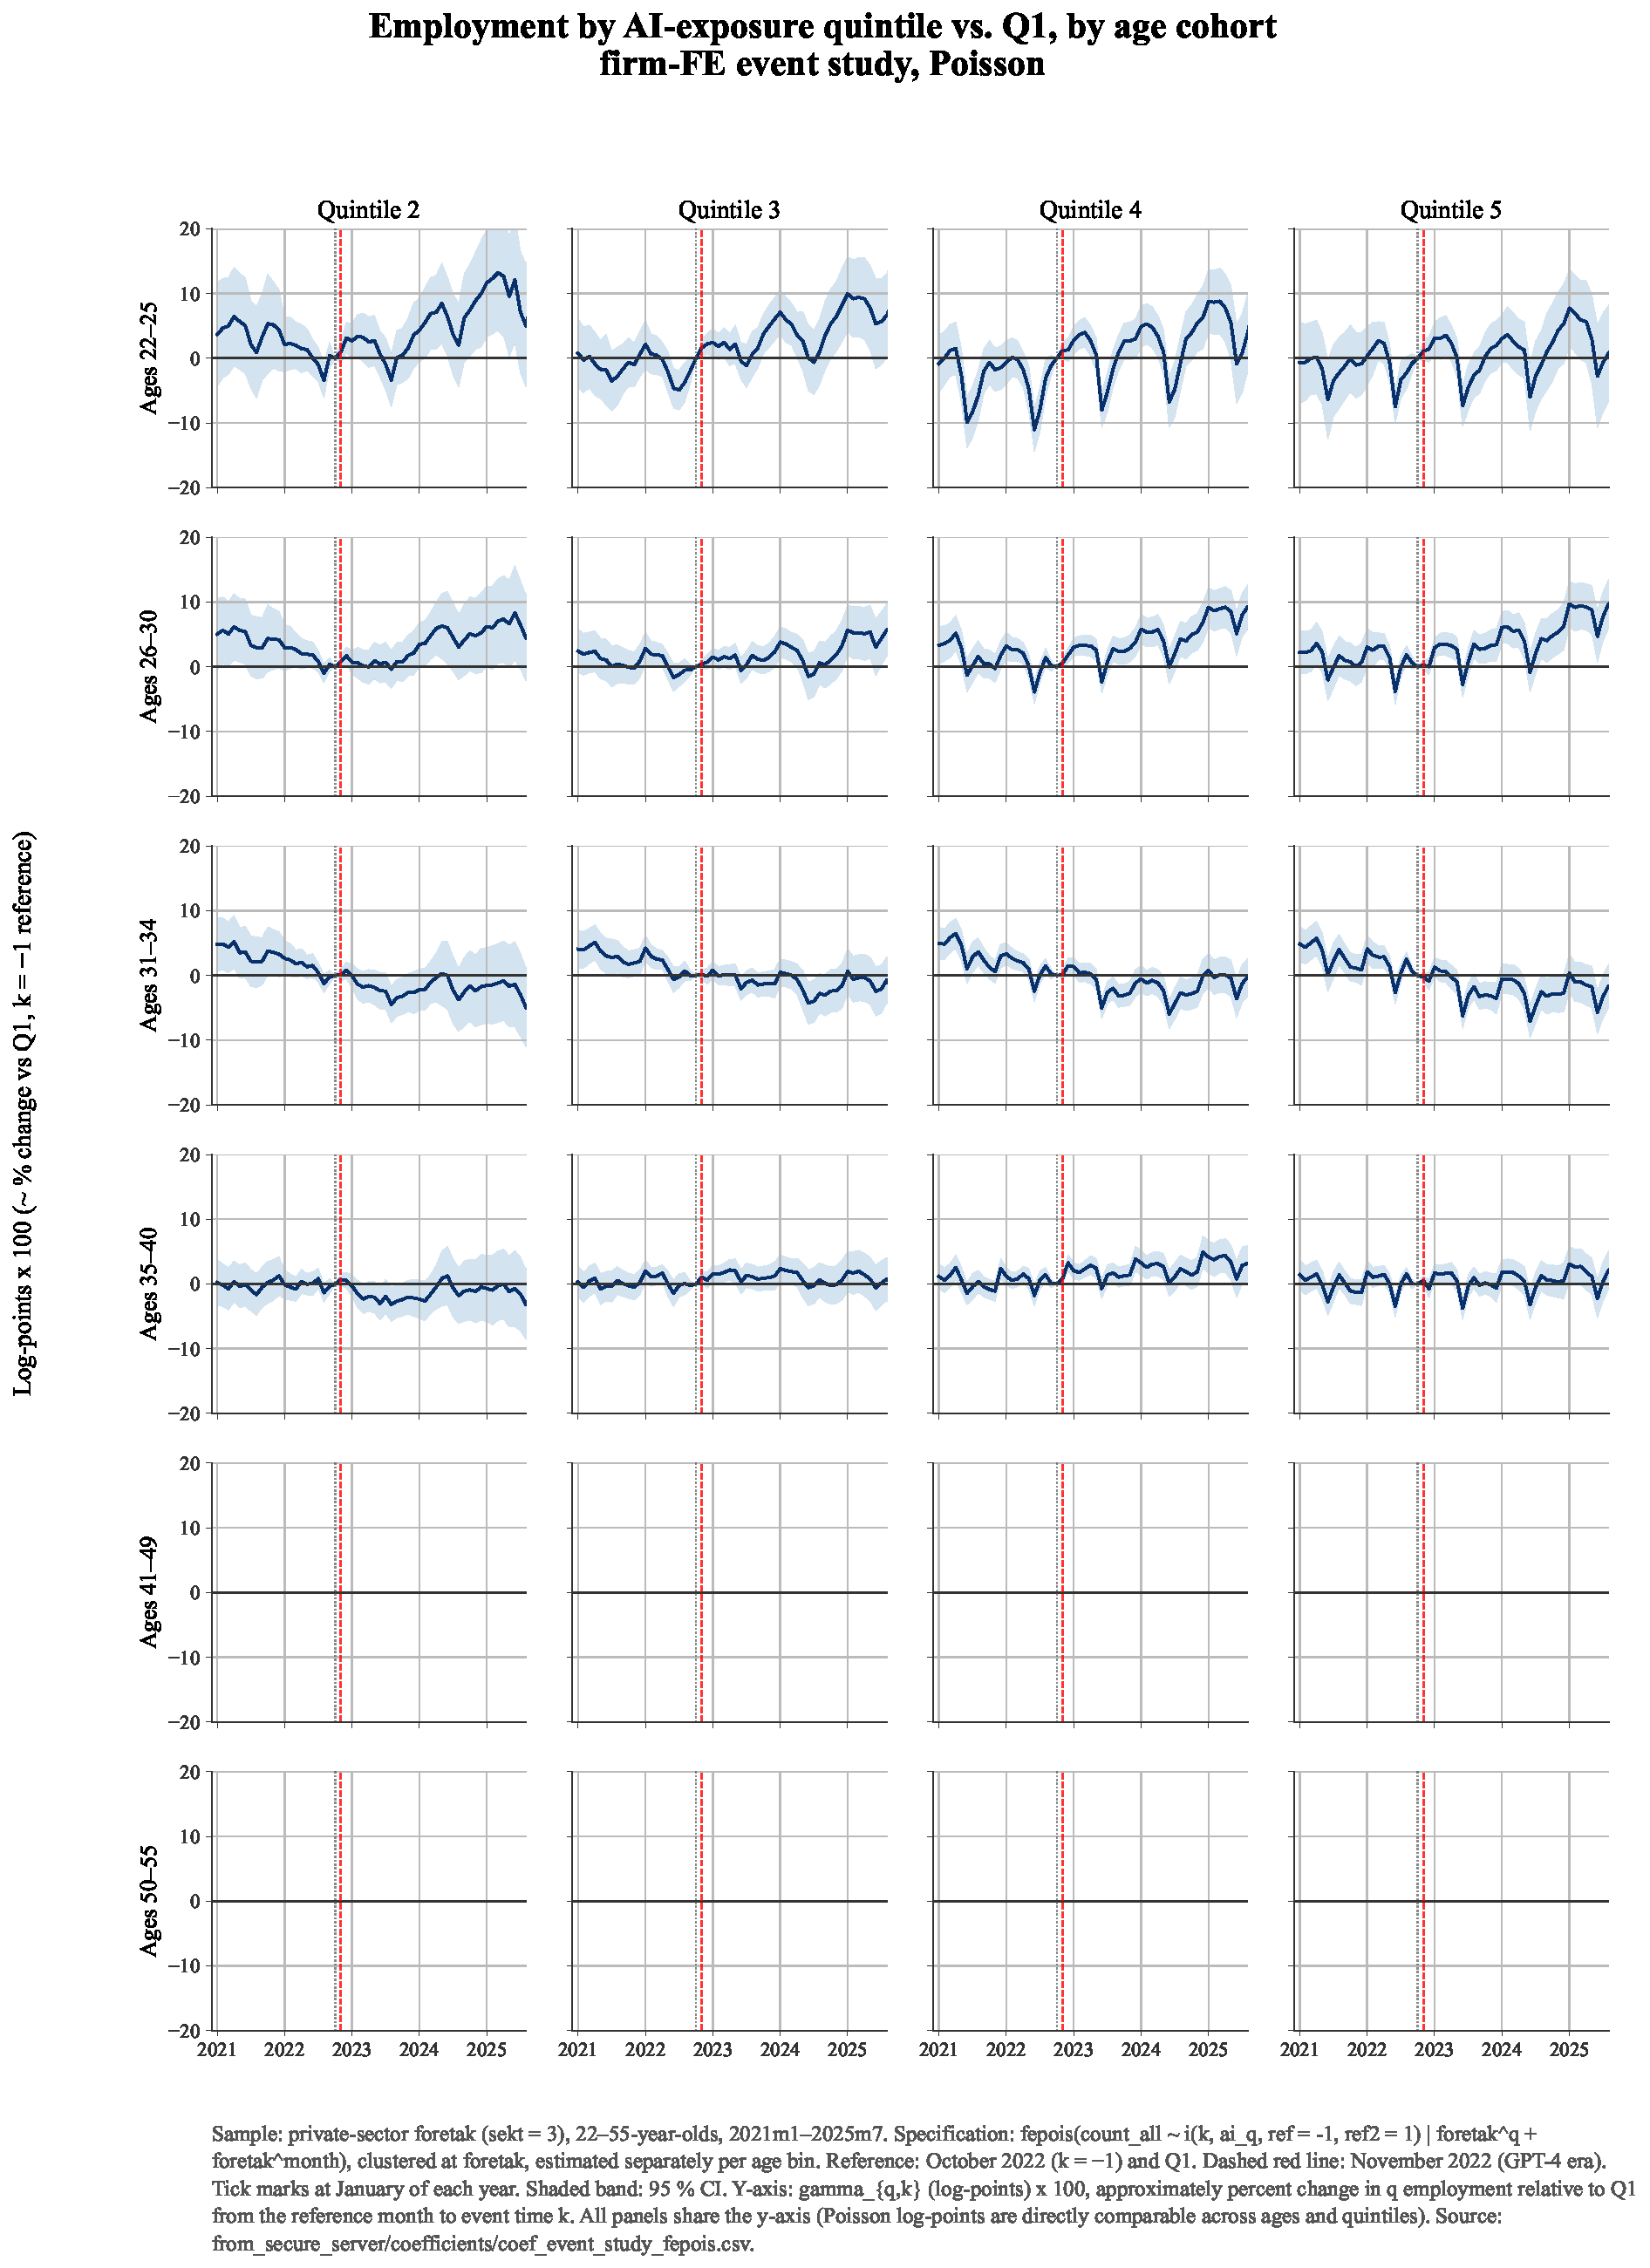
\includegraphics[width=\textwidth]{../analysis/output/figures/firm_fe_es_q2to5_grid_poisson.pdf}
  \caption{Poisson event-study coefficients $\gamma_{q,k}$ for $q\in\{2,\dots,5\}$ vs.\ $q=1$, by age bin. Individual-level employer-reported records, private-sector firms, ages 22--55, 2021m1--2025m7; FE: firm\,$\times$\,quintile and firm\,$\times$\,month. Shaded band: 95\% CI clustered at firm. Reference: October 2022. Dashed red line: November 2022.}
  \label{fig:firmfe_poisson_grid}
\end{figure}

\paragraph{Interpretation.}
The cell-level analysis counts every worker in the formal economy and so picks up the cohort-level decline that drives the linear rate figures. The firm-FE analysis sees only the panel of private-sector firms with at least 20 workers in the age window throughout 2021m1--2025m7, and within those firms it estimates how the Q5 vs.\ Q1 mix of young workers evolves over time. A firm-FE coefficient on Q5 22--25 close to zero therefore says only that the young Q5/Q1 mix is roughly unchanged \emph{within} the firms that meet the panel restriction, it is silent about firms that shrank below the size cutoff, exited, or were never in private employment, and about new firms that entered after 2021. One potential reading of a sharp cell-level decline combined with a near-zero firm-FE coefficient is that the cohort-level fall operates between firms rather than through reorganization inside continuing firms: Q5-exposed firms may be growing more slowly (or shrinking, exiting, failing to be replaced) relative to Q1-exposed firms, while each surviving firm's internal mix of young workers across exposure quintiles stays roughly the same. The mid-career positive coefficients from the firm-FE specification go further and imply that continuing firms reweight toward exposed occupations among workers in their early thirties to early forties.

Table~\ref{tab:firmfe_alt} reports the pooled young\,$\times$\,post\,$\times$\,exposure\_std triple-difference: Under the firm-FE Poisson regression, the coefficient is $-0.0022$ (SE $0.0063$); the linear-OLS analogue on the count is $-0.0058$ (SE $0.0104$). Within the same firm and month, young workers in higher-exposure occupations do not decline relative to older ones in the same firm. The cohort-level decline therefore appears to run through the extensive margin (which firms hire young workers, and which young workers find employment at all) rather than through reshuffling of young workers across exposure quintiles inside continuing firms.

\paragraph{Intensive margin.}
Table~\ref{tab:firmfe_alt} brings the extensive-margin pooled triple-differences together with the intensive-margin outcomes. The intensive-margin rows are linear-OLS triple-differences with firm-by-age, firm-by-month, and age-by-month fixed effects, weighted by cell employment. The reported coefficient is on young\,$\times$\,post\,$\times$\,exposure\_std: the differential post-October-2022 response for 22--25 year-olds relative to older workers in the same firm and month, per one standard deviation of occupational exposure. After October 2022, a one standard deviation increase in exposure is associated with a 0.8 percent lower monthly wage and a 0.4 percentage point lower contracted position percentage for 22--25 year-olds relative to older workers within the same firm. Base hours and overtime are unchanged. The intensive-margin magnitudes are small and would not appear in the quintile-level series of Section~\ref{sec:results:wages}, but they go in the same direction as the extensive-margin findings.

\begin{table}[htbp]
  \centering
  \caption{Pooled triple-difference estimates, firm-FE specification.}
  \label{tab:firmfe_alt}
  \begin{tabular}{lccc}
  \toprule
  Outcome & Coef. & SE & $t$ \\
  \midrule
  \multicolumn{4}{l}{\textit{Extensive margin (employment count)}} \\
  Headcount, Poisson (log points)        & $-0.0022$ & $0.0063$ & $-0.34$ \\
  Headcount, linear OLS                  & $-0.0058$ & $0.0104$ & $-0.55$ \\
  \midrule
  \multicolumn{4}{l}{\textit{Intensive margin}} \\
  Log monthly wage                       & $-0.0077$ & $0.0022$ & $-3.50$ \\
  Position pct                           & $-0.396$  & $0.099$  & $-4.02$ \\
  Log base hours                         & $-0.0027$ & $0.0027$ & $-1.00$ \\
  Overtime hours                         & $-0.011$  & $0.027$  & $-0.43$ \\
  \bottomrule
  \end{tabular}
  \\[3pt]
  \footnotesize Coefficient on young\,$\times$\,post\,$\times$\,exposure\_std. All rows use firm\,$\times$\,age + firm\,$\times$\,month + age\,$\times$\,month fixed effects. Extensive-margin rows (Poisson and linear OLS on the count) are unweighted; intensive-margin rows are weighted by cell employment so the cell-level OLS reproduces the underlying individual-level regression. SE clustered at firm.
\end{table}
